\subsection{Debugger}\label{debugger}
The validation of the codegen lead to another validation-issue.
If a test program is not behaving as expected, is there a bug in the test program or in the compiler?

In other words:

\textit{How to validate the test programs?}

The answer to this is an embedded debugger in the target executable.

\fbox{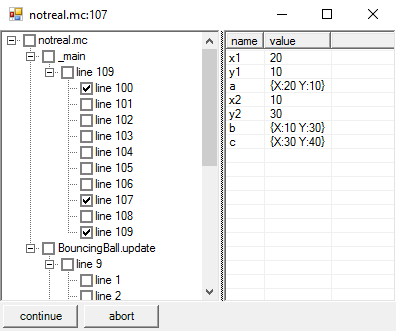
\includegraphics[width=\columnwidth-7pt]{debugger}}

%The backend can also embed an interactive debugger in the codegen.
The program will then trigger a breakpoint on the first instruction and launch the debugger GUI.
From the GUI, more breakpoints can be set with the check-boxes.
When the user presses `continue' or `abort', the gui will close and appear again on the next breakpoint.

The left pane shows a four level deep tree which sorts the program on file name, function name, rule and line.

The right pane shows a table with the name and value of the local identifiers defined up to the current breakpoint.

\subsubsection{Program changes}
When compiling with the debug flag set, some additions are made to target program.

\paragraph{Local identifier table}
After each instruction that defines named local identifiers, a new instruction is generated.

\begin{code}
    var foo = 42;
    _DBUG_symbol_table["foo"] = foo;
\end{code}

After each assignment to a named local identifier, the named identifier and the value are recorded in a key-value collection. 
This key-value collection will be passed to the debugger when a breakpoint is hit.
A new key-value collection is defined at the start of each rule.

\paragraph{Break points}
When compiling with the debug-flag set, function closures will have a group of boolean arrays.
One array for each rule in the function.

\begin{code}
    class <function name>{
        <arguments>
        static bool[] _DBUG_breakpoints_0;
        static bool[] _DBUG_breakpoints_1;
        <return value> _run(<last argument>){
            <body> 
        }
    }
\end{code}

The breakpoints are generated at each line of sourcecode in the rule.
This is different than breaking at every instruction, as normalization often splits single lines into multiple instructions.

\begin{code}
    ...
    if(_DBUG_Breakpoints_1[6]){
        _DBUG.breakpoint("filename.mc", 12, 
                         _DBUG_symbol_table);
    }
    ...
\end{code}

\subsubsection{Debug class}
The breakpoint function is defined as a public static member of the debug class.

The debugger is defined in a seperate file, \verb|_DBUG.cs|, which is imported by the target executable.
This is done to keep the program-specific code out of \verb|_DBUG.cs|.

\verb|_DBUG.cs| contains the class \verb|_DBUG|.
This class contains only the following public static items.

\begin{enumerate}
    \item the program tree
    \item the breakpoint tree
    \item the breakpoint function
\end{enumerate}

The program builds up the program tree and the breakpoint tree in the main function, before the first user-written line starts.
The trees are both four-levels deep and sorted on filename, function name, rule and linenumber.
The breakpoint function is called when the program hits a break-point.

This was chosen because breakpoint checks happen every few instructions, so they have a huge effect on debug performace.
Straight arrays with booleans are very fast to index since it only costs one bounds-check, one addition and one dereference.

\paragraph{The tree representation} of the program is four levels deep.
The first level represents the file, the second level represents the funcion, the third level represents the rule and the fourth level represents the premise.

\paragraph{The breakpoint table} 
Breakpoints are realised as an array of booleans for each rule in a closure.
The class also contains a \verb|bool[][][][]| 

\paragraph{The breakpoint function}
This class contains a static method \verb|breakpoint| that will pause the execution of the program and present the GUI.
When the user presses `continue' or `abort', the GUI will close and the \verb|breakpoint| method will return control back to the program.

The first two arguments to \verb|_DBUG.breakpoint| are the filename and the linenumber.
This is to uniquely identify the callsite.
The third argument is the symboltable that has been accumulated so far.

\subsubsection{Initialization}
The program tree is a public field of the \verb|_DBUG| class, and is initialized by the main function.

\subsubsection{Evolution}
First own tree impl.
Then 4d node.
Now winform tree nodes.

